

%\documentclass{book}\begin{document}<content\end{document}
\documentclass[letter, 11pt]{texMemo}  % The texMemo package by Rob Oakes.

\usepackage{amsmath}
\usepackage[colorlinks=true, citecolor=blue]{hyperref}
\usepackage{enumitem}
\usepackage{graphicx, lipsum}

\usepackage[LGRgreek]{mathastext}

\usepackage{natbib}
\bibliographystyle{apalike}


\memodate{\today~(Submitted)}
%\memoto{Dr. Dan Russell - College of Engineering, Penn State University}
%\memofrom{Michael R. Wirtzfeld - Sound Discovery LLC\\}
\memosubject{ACS 597 - Module 1 Assignement\\}

%\memologo{
\includegraphics[width=1.0\textwidth]{SOUND_DISCOVERY_Business_Card.jpg}}



\begin{document}

\maketitle



\subsection*{Problem 1a}

The lowest cut-on frequency for a rectangular duct with air flow is given by equation,

\vspace{-0.25cm}
\begin{equation}
    f_{cut-on} = 0.5 \cdot \frac{c}{L}
\end{equation}

where $c$ is the speed of sound in air, 343~$\frac{m}{s}$,  and $L$ is the largest side of the rectangular cross-section.

\vspace{0.25cm}
With cross-sectional dimensions of $L_x = 12~cm$ and $L_y = 20~cm$, the lowest cut-on frequency for this rectangular duct is,

\vspace{-0.25cm}
\begin{equation*}
    f_{cut-on} = 0.5 \cdot \frac{ 343~\frac{m}{s} }{ 0.20~m } = \boldsymbol{857.5~Hz}
\end{equation*}




\subsection*{Problem 1b}

The lowest cut-on frequency for a circular duct with air flow with the same cross-sectional area as the rectangular duct in part (a.) can be calculated using equation,

\vspace{-0.25cm}
\begin{equation}
    f_{cut-on} = 0.568 \cdot \frac{c}{d}
    \label{equation:circularDuct}
\end{equation}

where $c$ is the speed of sound in air, 343~$\frac{m}{s}$,  and $d$ is diameter of the circular duct.

\vspace{0.25cm}
The cross-sectional area of the rectangular duct is,

\vspace{-0.25cm}
\begin{equation*}
    Area_{~rectangular~duct} = 0.12~m~\cdot0.20~m =  0.024~m
\end{equation*}

\vspace{0.25cm}
The corresponding diameter for this area is,

\vspace{-0.25cm}
\begin{equation*}
    diameter = \sqrt{ \frac{0.24~m^2}{\pi} } \cdot 2 = 0.17~m
\end{equation*}

\vspace{0.25cm}
Using Eq.~\ref{equation:circularDuct}, the lowest cut-on frequency for this circular duct with air flow is,

\vspace{-0.25cm}
\begin{equation*}
    f_{cut-on} = 0.568 \cdot \frac{ 1,500~\frac{m}{s} }{ 0.17~m } = \boldsymbol{1,114.5~Hz}
\end{equation*}





\subsection*{Problem 1c}

The lowest cut-on frequency for this circular duct with water flow can be calculated using Eq.~\ref{equation:circularDuct},

\vspace{-0.25cm}
\begin{equation*}
    f_{cut-on} = 0.568 \cdot \frac{ 1,500~\frac{m}{s} }{ 0.17~m } = \boldsymbol{4,873.9~Hz}
\end{equation*}

The lowest cut-on frequency for water is considerable larger than it is for air flow.





\newpage
\subsection*{Problem 1d}

The speed of sound in air is calculated by,

\vspace{-0.25cm}
\begin{equation}
    c = \sqrt{ \gamma \cdot R \cdot T_K }
    \label{equation:speedOfSoundInAir}
\end{equation}

where $\gamma$ is the ratio of specific heats, $R = 287~\frac{J}{kg \cdot K}$ is the gas constant, and $T_K$ is the absolute temperature in Kelvin.


speed of sound in air, 343~$\frac{m}{s}$,  and $d$ is diameter of the circular duct.




\vspace{-0.5cm}
\begin{figure}[!htb]

    \center
        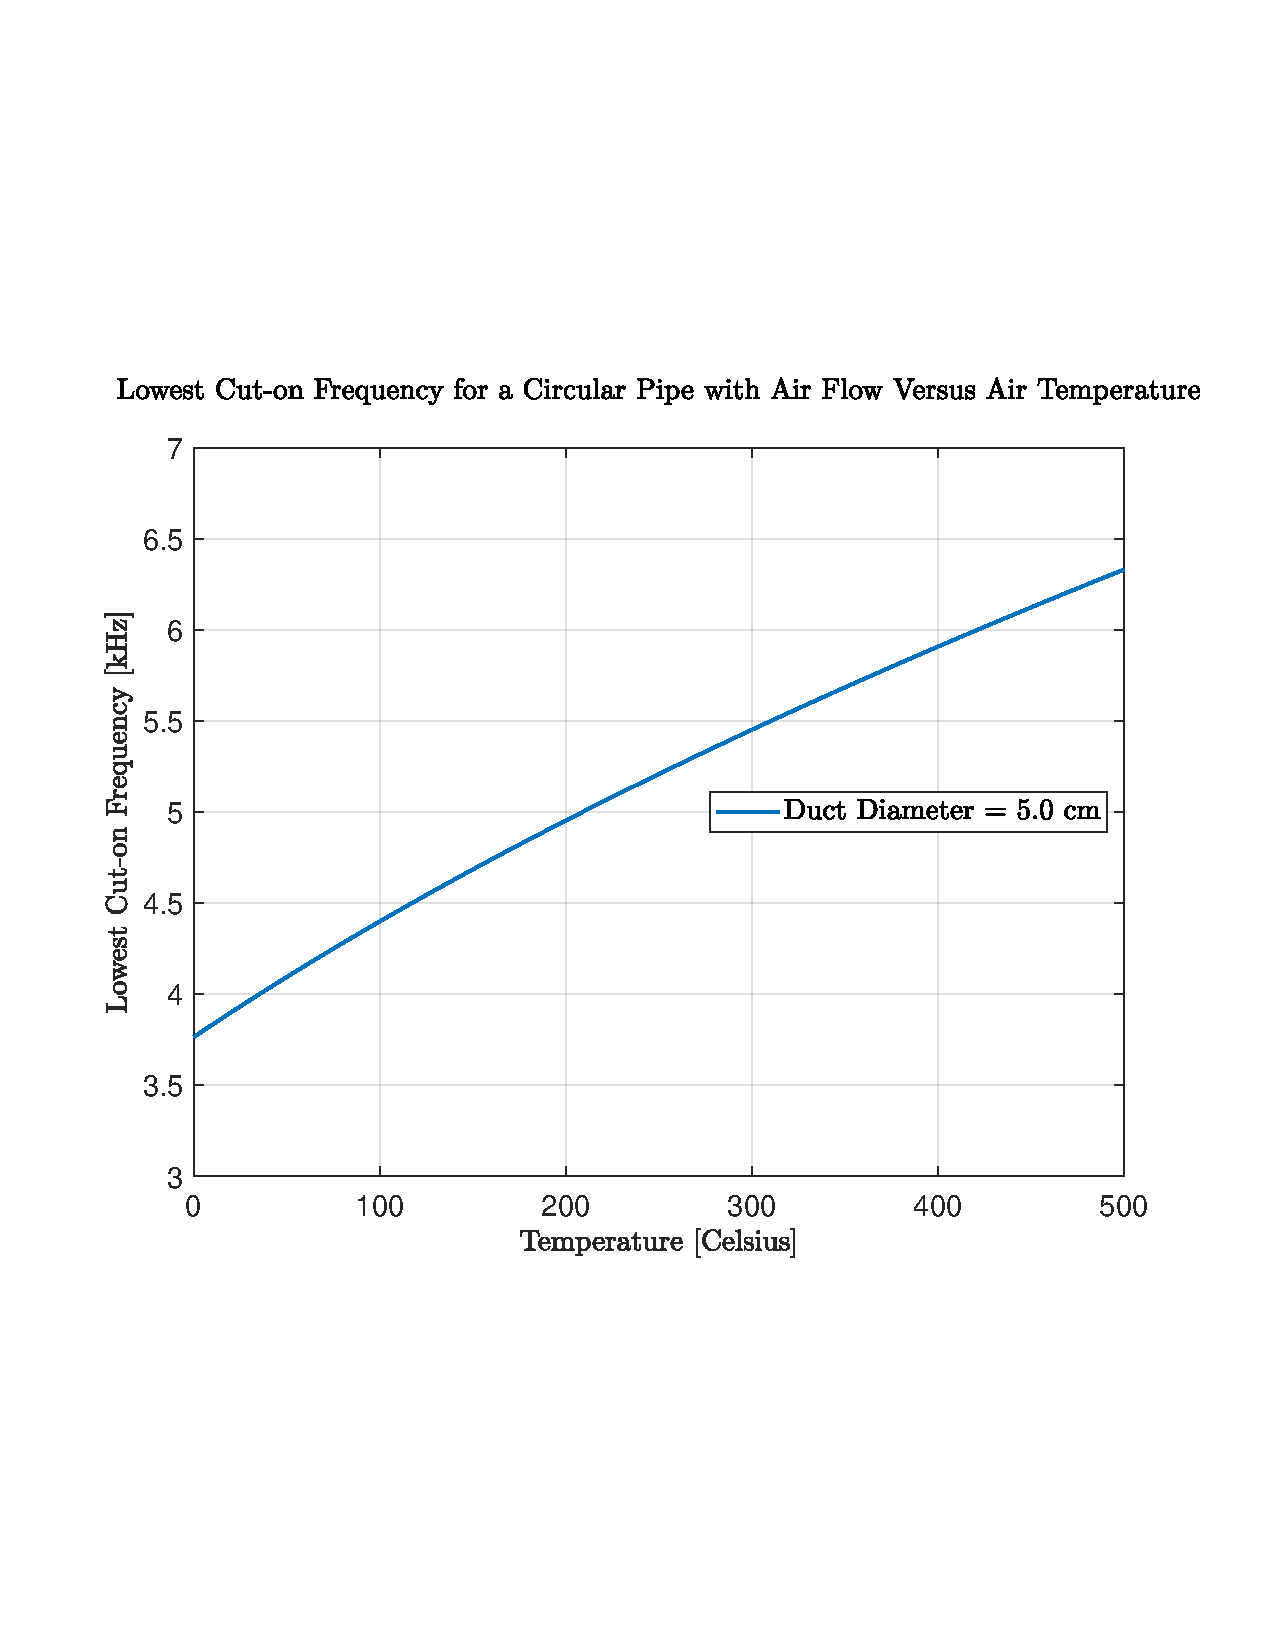
\includegraphics[ scale = 0.8, keepaspectratio ]{Cut-on Frequency Versus Temperature - Sunday, January 19, 2025.pdf}

    \vspace{-5.2cm}
    \caption{ph.}
    \label{figure:cuton_frequency_versus_temperature}

\end{figure}






\subsection*{Problem 1e}


% Question:  Are cut-on frequencies higher for a circular or rectangular duct for a given cross-sectional area?

% The lowest cut-on frequency is higher for a circular duct than for a
% rectangular duct for a given cross-sectional area.

% For the dimensions given in class, the rectangular duct is not square.
% This produces a larger dimension and thus a smaller, lowest cut-on
% frequency.

% If the rectangular duct is square dimensions on the order of the circular
% duct diameter with the same cross-sectional area, the the cut-on
% frequencies are approximately equal.


% Question:  What about in air versus water?

% The lowest cut-on frequency is larger with water than air.  This due to
% the fact that the cut-on frequency is proportional to the speed of sound
% and the speed of sound in water is greater than it is in air.


% Question:  What about cold versus hot air?

% For a circular pipe, the cut-on frequency is higher in warm air than cold
% air.





\end{document}


































